\documentclass[11pt]{extbook}
% Builds with:
% xelatex testplan.tex

\usepackage{style}
\usepackage{enumitem}
\usepackage{titling}
\usepackage{listings}
\usepackage{color}
\usepackage{multicol}
\newcommand\tab[1][1cm]{\hspace*{#1}}
\usepackage[utf8]{inputenc}
\usepackage{pdflscape}
\usepackage{changepage}
\usepackage{float}
\graphicspath{ {./} }


\title{%
\begin{tabular}{cl}
PROJECT `dungeon\_dudes'\tabularnewline
\large Design\tabularnewline
\large MOD O - OOP 2B\tabularnewline
\small 170D WOBC\tabularnewline
\small Class 23-001\tabularnewline
\end{tabular}
}
\subtitle{\large dungeon\_dudes}

\author{%
\begin{tabular}{cl}
WO1 Josh Kaplan
\end{tabular}
}
\date{\today}

\begin{document}

\maketitle

\section*{\emph{1 Purpose}}

\tab The project \emph{dungeon\_dudes} is an object-oriented program in Python 
which are to create a Character or Monster for a Dungeon-Crawler style RPG
in accordance with an already existing codebase. The Character or Monster must
match the associated Character Stats and information found in the Manual for 
Dungeon Dudes. This is in order to teach us the appropriate way to integrate 
work into an existing codebvase and master the art of git collaboration. 

\section*{\emph{2 Design}}

\tab The design for the Cleric \emph{dungeon\_dudes} is relatively 
straight-forward, as we simply just need to follow the character sheet.

\tab Using the Fighter CharacterClass as reference, we create a BaseClass for
the required item generation with the correct or slightly modified values to 
match the Cleric. Most of the code can be appropriated.

\tab For the Cleric CharacterClass itself, the \emph{\_\_init\_\_} values from 
Fighter carry over as well, with modified values for levels and stats. 
Additional bools are created to track the different skills for half damage, no 
damage, etc. The modifiers for Offense and Defense carry over as well. 

\tab Afterwards, we create class methods unique to the cleric: 
\verb|divine_blessing|, \verb|improved_healing|, \verb|heal|,
\verb|radiance|, \verb|prayer|, \verb|avenger|, and
\verb|greater_heal|. These are written in line with the Character Sheet found 
in the Guide adoc.

\tab \verb|level_up| is mostly the same, except for the values to match the 
given Character Sheet

\tab \verb|take_damage| requires the most modification compared to the 
Fighter CharacterClass, as most of the special Passive skills are calculated
and tabulated within \verb|take_damage|.

\tab \verb|win_battle| is essentially a reset and is largely unchanged except 
for resetting our Cleric's bools for Passives and Special Abilities. Any other
methods needed from the Fighter CharacterClass carry over verbatim with no 
issues.

\section*{\emph{3 Diagrams}}

\tab For additional points of reference, the Fighter CharacterClass is included as
a point of comparison to the implementation of the Cleric CharacterClass.

\begin{figure}[H]
    \centering
    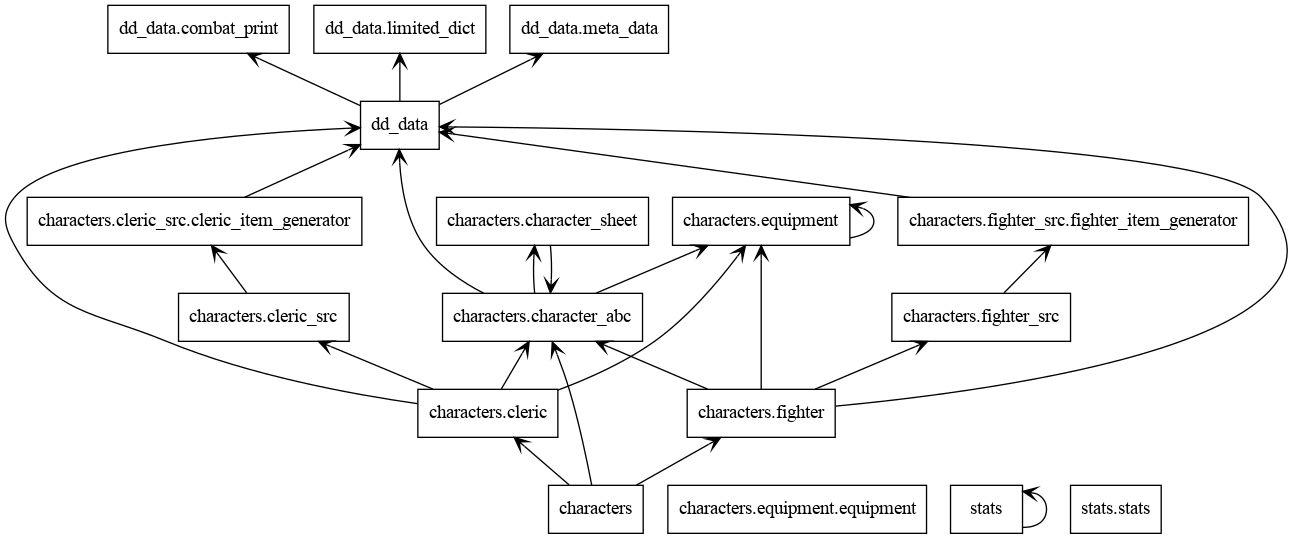
\includegraphics[scale=0.35]{01_packages_cleric}
    \caption{Packages diagram for the Cleric in \emph{dungeon\_dudes}}
\end{figure}

\newpage
\begin{landscape}

\begin{figure}[H]
    \centering
    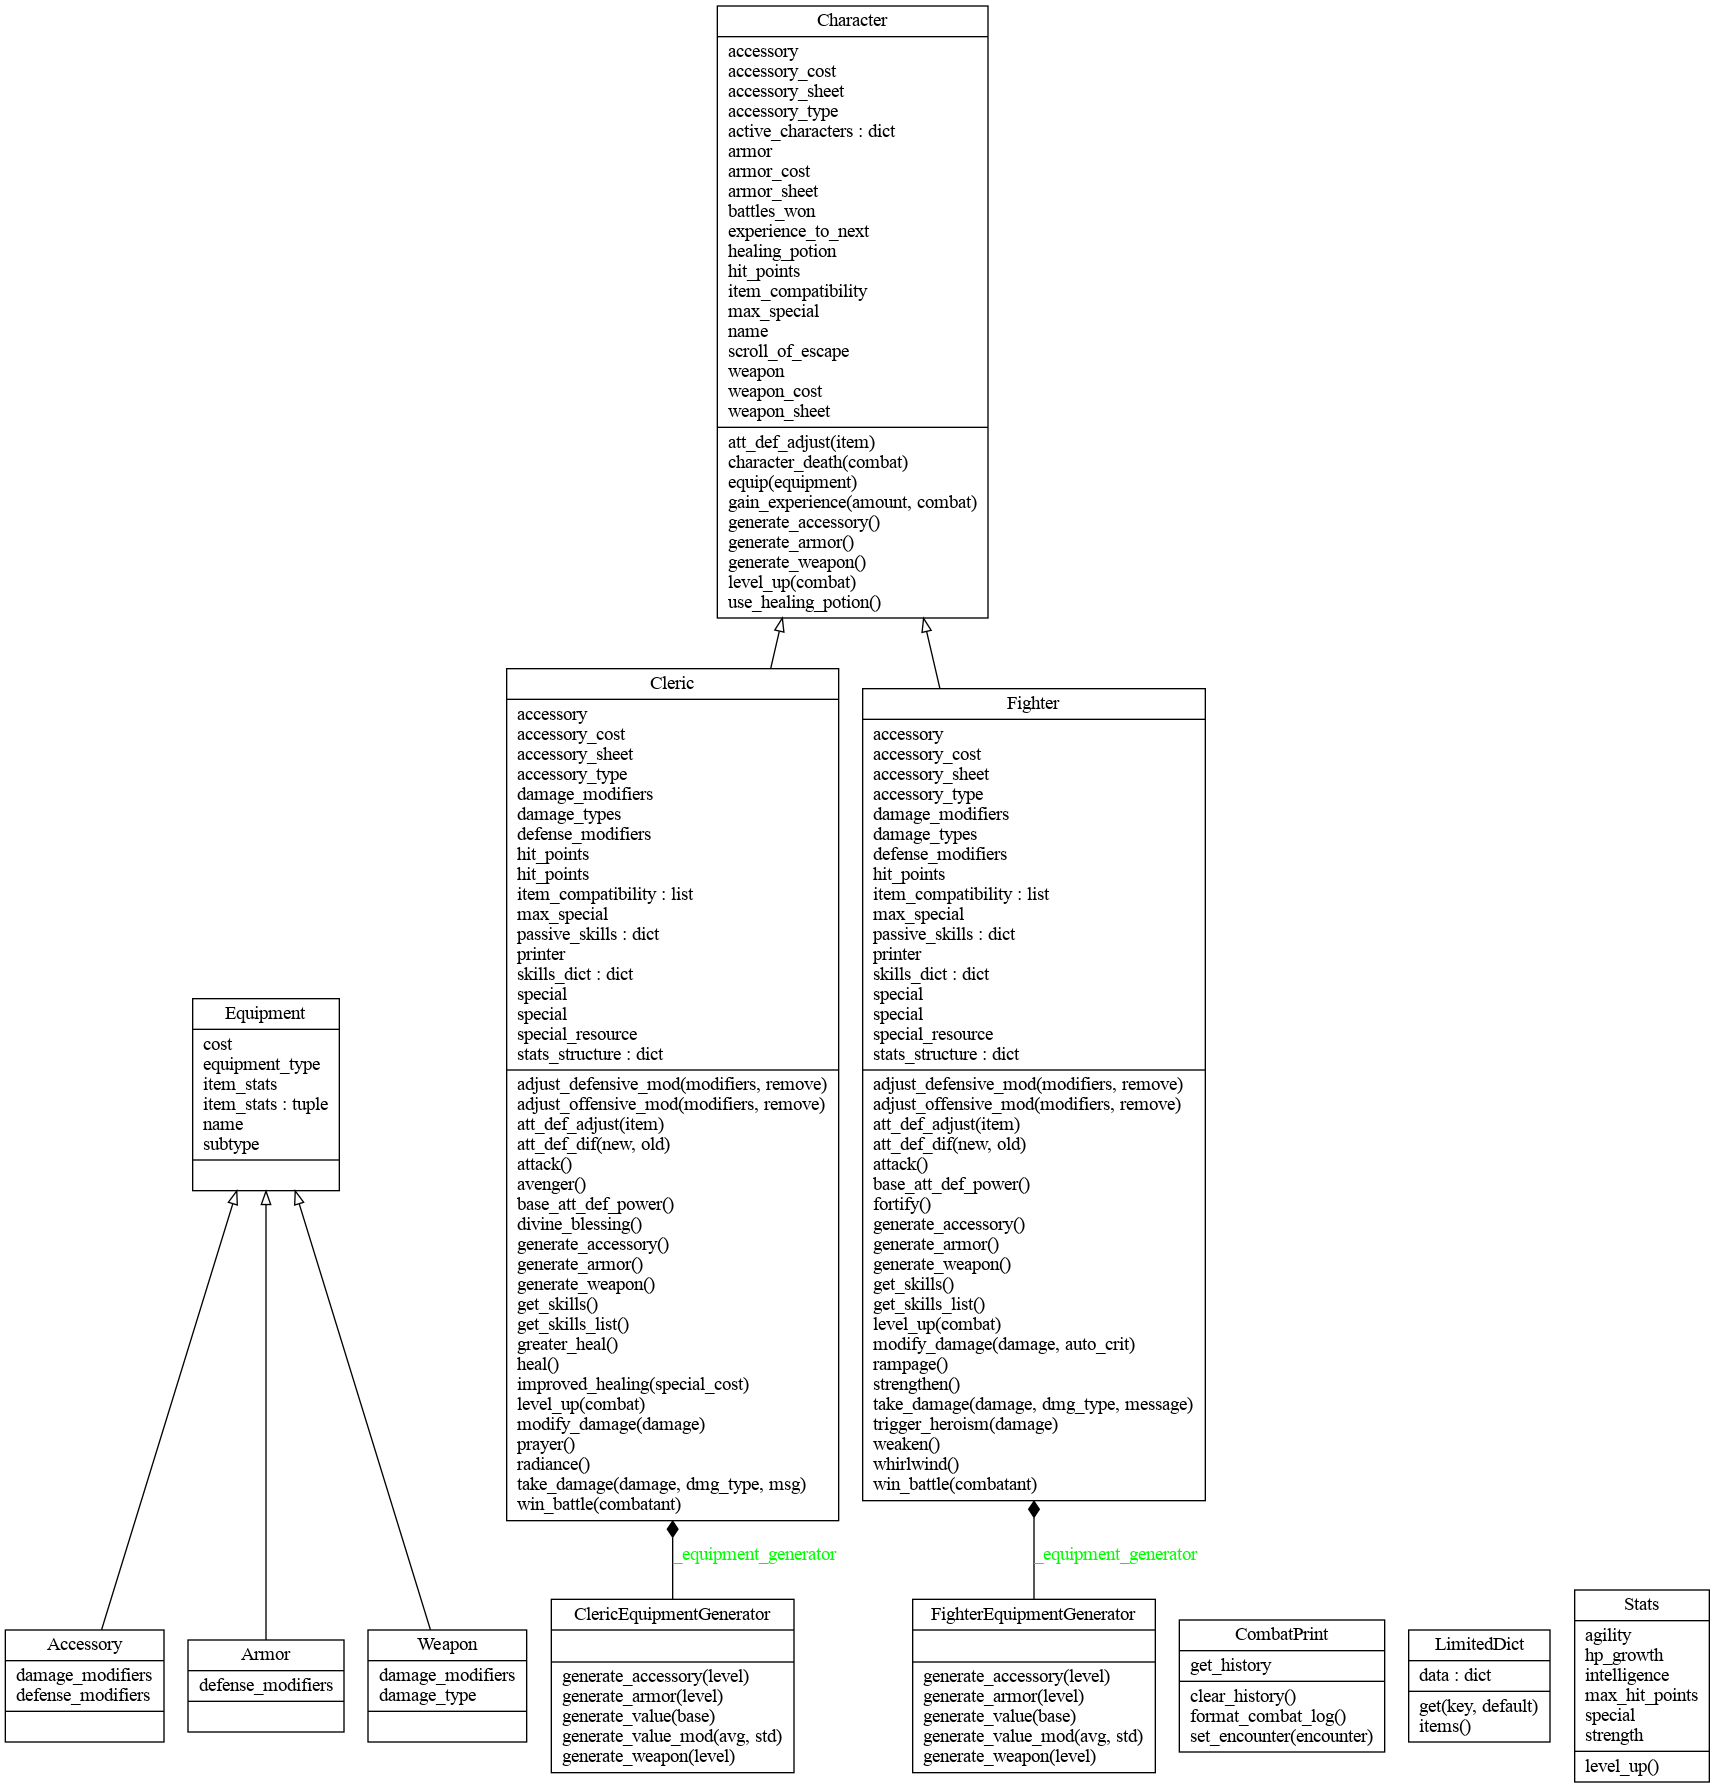
\includegraphics[scale=0.24]{02_classes_cleric}
    \caption{Classes diagram for the Cleric in \emph{dungeon\_dudes}}
\end{figure}

\end{landscape}

\end{document}
